
\documentclass[10pt,letterpaper]{article}
\usepackage[top=0.85in,left=2.75in,footskip=0.75in]{geometry}

% % % % % % % % % % % % % % % % % % % % % % % %

% Extra symbols added
\usepackage{stix}
%Three part table - I think this is allowed
\usepackage[flushleft]{threeparttable}

% % % % % % % % % % % % % % % % % % % % % % % %


% amsmath and amssymb packages, useful for mathematical formulas and symbols
\usepackage{amsmath} %amssymb

% Use adjustwidth environment to exceed column width (see example table in text)
\usepackage{changepage}

% Use Unicode characters when possible
\usepackage[utf8x]{inputenc}

% textcomp package and marvosym package for additional characters
\usepackage{textcomp,marvosym}

% cite package, to clean up citations in the main text. Do not remove.
\usepackage{cite}

% Use nameref to cite supporting information files (see Supporting Information section for more info)
\usepackage{nameref,hyperref}

% line numbers
\usepackage[right]{lineno}

% ligatures disabled
\usepackage{microtype}
\DisableLigatures[f]{encoding = *, family = * }

% color can be used to apply background shading to table cells only
\usepackage[table]{xcolor}

% array package and thick rules for tables
\usepackage{array}

% create "+" rule type for thick vertical lines
\newcolumntype{+}{!{\vrule width 2pt}}

% create \thickcline for thick horizontal lines of variable length
\newlength\savedwidth
\newcommand\thickcline[1]{%
  \noalign{\global\savedwidth\arrayrulewidth\global\arrayrulewidth 2pt}%
  \cline{#1}%
  \noalign{\vskip\arrayrulewidth}%
  \noalign{\global\arrayrulewidth\savedwidth}%
}

% \thickhline command for thick horizontal lines that span the table
\newcommand\thickhline{\noalign{\global\savedwidth\arrayrulewidth\global\arrayrulewidth 2pt}%
\hline
\noalign{\global\arrayrulewidth\savedwidth}}


% Remove comment for double spacing
%\usepackage{setspace} 
%\doublespacing

% Text layout
\raggedright
\setlength{\parindent}{0.5cm}
\textwidth 5.25in 
\textheight 8.75in

% Bold the 'Fig #' in the caption and separate it from the title/caption with a period
% Captions will be left justified
\usepackage[aboveskip=1pt,labelfont=bf,labelsep=period,justification=raggedright,singlelinecheck=off]{caption}
\renewcommand{\figurename}{Fig}

% Use the PLoS provided BiBTeX style
\bibliographystyle{plos2015}

% Remove brackets from numbering in List of References
\makeatletter
\renewcommand{\@biblabel}[1]{\quad#1.}
\makeatother

% Leave date blank
\date{}

% Header and Footer with logo
\usepackage{lastpage,fancyhdr,graphicx}
\usepackage{epstopdf}
\pagestyle{myheadings}
\pagestyle{fancy}
\fancyhf{}
\setlength{\headheight}{27.023pt}
\lhead{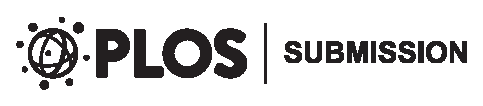
\includegraphics[width=2.0in]{PLOS-submission.eps}}
\rfoot{\thepage/\pageref{LastPage}}
\renewcommand{\footrule}{\hrule height 2pt \vspace{2mm}}
\fancyheadoffset[L]{2.25in}
\fancyfootoffset[L]{2.25in}
\lfoot{\sf PLOS}
%% Include all macros below

\newcommand{\lorem}{{\bf LOREM}}
\newcommand{\ipsum}{{\bf IPSUM}}

%reference equations in appendices
\usepackage{xr}
\externaldocument{main_revised}
\externaldocument{S2Appendix_revised}
\externaldocument{S3Appendix_revised}

%% END MACROS SECTION

\begin{document}
\vspace*{0.2in}

\setcounter{equation}{0}
\renewcommand{\theequation}{S1.\arabic{equation}}

\section*{S1 Appendix}

\subsection*{Recursion equations}


In each generation we census the genotype frequencies in male and female gametes/gametophytes (hereafter, gametes) between meiosis (and any meiotic drive) and gametic competition. 
At this stage we denote the frequencies of X- and Y-bearing gametes from males and females $x_{i}^{\circ}$ and $y_{i}^{\circ}$.
The superscript $\circ \in \{\male,\female\}$ specifies the sex of the diploid that the gamete came from. 
The subscript $i\in\{1,2,3,4\}$ specifies the genotype at the selected locus $\mathbf{A}$ and at the novel sex-determining locus $\mathbf{M}$, where $1=AM$, $2=aM$, $3=Am$, and $4=am$. 
The gamete frequencies from each sex sum to one, $\sum_{i}x_{i}^{\circ}+y_{i}^{\circ}=1$. 

Competition then occurs among gametes of the same sex (e.g., among eggs and among sperm separately) according to the genotype at the $\mathbf{A}$ locus ($w_{1}^\circ=w_{3}^\circ=w_{A}^\circ$, $w_{2}^\circ=w_{4}^\circ=w_{a}^\circ$, see Table \ref{tab:fitnesstable}).
The genotype frequencies after gametic competition are $x_{i}^{\circ,s}= w_{i}^{\circ}x_{i}^{\circ}/\bar{w}_{H}^{\circ}$ and $y_{i}^{\circ,s}= w_{i}^{\circ}y_{i}^{\circ}/\bar{w}_{H}^{\circ}$, where $\bar{w}_{H}^{\circ}=\sum_{i} w_{i}^{\circ}x_{i}^{\circ}+w_{i}^{\circ}y_{i}^{\circ}$ is the mean fitness of male ($\circ=\male$) or female ($\circ=\female$) gametes. 

Random mating then occurs between gametes to produce diploid zygotes.
%To shorten notation we now use index $i$ (and $j$) to denote the alleles at both the $\mathbf{A}$ and $\mathbf{M}$ loci and label $MA=1$, $Ma=2$, $mA=3$, and $ma=4$, such that $i,j\in\{1,2,3,4\}$.
The frequencies of XX zygotes are then denoted as $xx_{ij}$, XY zygotes as $xy_{ij}$, and YY zygotes as $yy_{ij}$, where $\mathbf{A}$ and $\mathbf{M}$ locus genotypes are given by $i,j\in\{1,2,3,4\}$, as above. 
In XY zygotes, the haplotype inherited from an X-bearing gamete is given by $i$ and the haplotype from a Y-bearing gamete is given by $j$. 
In XX and YY zygotes, individuals with diploid genotype $ij$ are equivalent to those with diploid genotype $ji$; for simplicity, we use $xx_{ij}$ and $yy_{ij}$ with $i\neq j$ to denote the average of these frequencies, $xx_{ij}=(x_{i}^{\female,s}x_{j}^{\male,s}+x_{j}^{\female,s}x_{i}^{\male,s})/2$ and $yy_{ij}=(y_{i}^{\female,s}y_{j}^{\male,s}+y_{j}^{\female,s}y_{i}^{\male,s})/2$. 


Denoting the $\mathbf{M}$ locus genotype by $b \in \{MM, Mm, mm\}$ and the $\mathbf{X}$ locus genotype by $c \in \{XX, XY, YY\}$, zygotes develop as females with probability $k_{bc}$. 
Therefore, the frequencies of XX females are given by $xx_{ij}^{\female}=k_{bc}xx_{ij}$, XY females are given by $xy_{ij}^{\female}=k_{bc}xy_{ij}$, and YY females are given by $yy_{ij}^{\female}=k_{bc}yy_{ij}$. 
Similarly, XX male frequencies are $xx_{ij}^{\male}=(1-k_{bc})xx_{ij}$, XY male frequencies are $xy_{ij}^{\male}=(1-k_{bc})xy_{ij}$, and YY males frequencies are $yy_{ij}^{\male}=(1-k_{bc})yy_{ij}$.
This notation allows both the ancestral and novel sex-determining regions to determine zygotic sex according to an XY system, a ZW system, or an environmental sex-determining system. 
In addition, we can consider any epistatic dominance relationship between the two sex-determining loci. 
Here, we assume that the ancestral sex-determining system ($\mathbf{X}$ locus) is XY ($k_{MMXX}=1$ and $k_{MMXY}=k_{MMYY}=0$) or ZW ($k_{MMZZ}=0$ and $k_{MMZW}=k_{MMWW}=1$) and epistatically recessive to a dominant novel sex-determining locus, $\mathbf{M}$ ($k_{Mmc}=k_{mmc}=k$). 


Selection among diploids then occurs according to the diploid genotype at the $\mathbf{A}$ locus, $l \in \{AA, Aa, aa\}$, for an individual of type $ij$ (see Table \ref{tab:fitnesstable}). 
The diploid frequencies after selection in sex $\circ$ are given by $xx_{ij}^{\circ,s}=w_{l}^{\circ} xx_{ij}/\bar{w}^{\circ}_{D}$, $xy_{ij}^{\circ,s}=w_{l}^{\circ} xy_{ij}/\bar{w}^{\circ}_{D}$, and $yy_{ij}^{\circ,s}=w_{l}^{\circ} yy_{ij}/\bar{w}^{\circ}_{D}$, where $\bar{w}^{\circ}_{D}= \sum_{i=1}^{4}\sum_{j=1}^{4}w_{l}^{\circ}xx_{ij}+w_{l}^{\circ}xy_{ij}+w_{l}^{\circ}yy_{ij}$ is the mean fitness of diploids of sex $\circ$. 

Finally, these diploids undergo meiosis to produce the next generation of gametes. 
Recombination and sex-specific meiotic drive occur during meiosis.
%We can also assume that recombination is sex specific and/or affected by the M locus - but generally we don't so I just describe $R=R_{f}=R, r_{MM,d}=r_{Mm,d}=r_{mm,d}=r, \chi_{m}=\chi_{f}=\chi$.
Here, we allow any relative locations for the $\mathbf{X}$, $\mathbf{A}$, and $\mathbf{M}$ loci by using three parameters to describe the recombination rates between them. 
$R$ is the recombination rate between the $\mathbf{A}$ and $\mathbf{M}$ loci, $\rho$ is the recombination rate between the $\mathbf{M}$ and $\mathbf{X}$ loci, and $r$ is the recombination rate between the $\mathbf{A}$ and $\mathbf{X}$ loci (Fig \ref{fig:model_outline}). 
\nameref{tab:chisubstitutions} shows replacements that can be made for each possible ordering of the loci assuming that there is no cross-over interference.
During meiosis in sex $\circ$, meiotic drive occurs such that, in $Aa$ heterozygotes, a fraction $\alpha^{\circ}$ of gametes produced carry the $A$ allele and $(1-\alpha^\circ)$ carry the $a$ allele. 

Among gametes from sex $\circ$, the frequencies of haplotypes (before gametic competition) in the next generation are given by

\begingroup
\allowdisplaybreaks
\begin{subequations}
\begin{align}
%
\begin{split}
x_{1}^{{\circ}'}=&xx_{11}^{\circ,s}+xx_{13}^{\circ,s}/2+(xx_{12}^{\circ,s}+xx_{14}^{\circ,s})\alpha^\circ\\
&-R(xx_{14}^{\circ,s}-xx_{23}^{\circ,s}) \alpha^\circ\\
&+(xy_{11}^{\circ,s}+xy_{13}^{\circ,s})/2+(xy_{12}^{\circ,s}+xy_{14}^{\circ,s})\alpha^\circ\\
&- r(xy_{12}^{\circ,s}-xy_{21}^{\circ,s})\alpha^\circ - \rho(xy_{13}^{\circ,s}-xy_{31}^{\circ,s})/2\\
&+\big{[}-(R+r+\rho)xy_{14}^{\circ,s} +(R+\rho-r)xy_{41}^{\circ,s}\\
&+(R+r-\rho) xy_{23}^{\circ,s}+(R+\rho-r)xy_{32}^{\circ,s}\big{]}\alpha^\circ/2
\end{split}
\\
%
\begin{split}
x_{2}^{{\circ}'}=&xx_{22}^{\circ,s}+xx_{24}^{\circ,s}/2+(xx_{12}^{\circ,s}+xx_{23}^{\circ,s})\alpha^\circ\\
&-R(xx_{23}^{\circ,s}-xx_{14}^{\circ,s}) \alpha^\circ\\
&(xy_{22}^{\circ,s}+xy_{24}^{\circ,s})/2+(xy_{21}^{\circ,s}+xy_{23}^{\circ,s})(1-\alpha^\circ)\\
&- r(xy_{21}^{\circ,s}-xy_{12}^{\circ,s})(1-\alpha^\circ) - \rho(xy_{24}^{\circ,s}-xy_{42}^{\circ,s})/2\\
&+\big{[}-(R+r+\rho)xy_{23}^{\circ,s}+(R+\rho-r)xy_{32}^{\circ,s}\\
&+(R+r-\rho) xy_{14}^{\circ,s}+(R+\rho-r)xy_{41}^{\circ,s}\big{]}(1-\alpha^\circ)/2
\end{split}
\\
%
\begin{split}
x_{3}^{{\circ}'}=&xx_{33}^{\circ,s}+xx_{13}^{\circ,s}/2+(xx_{23}^{\circ,s}+xx_{34}^{\circ,s})\alpha^\circ\\
&-R(xx_{23}^{\circ,s}-xx_{14}^{\circ,s}) \alpha^\circ\\
&(xy_{33}^{\circ,s}+xy_{31}^{\circ,s})/2+(xy_{32}^{\circ,s}+xy_{34}^{\circ,s})\alpha^\circ\\
&- r(xy_{34}^{\circ,s}-xy_{43}^{\circ,s}) \alpha^\circ - \rho(xy_{31}^{\circ,s}-xy_{13}^{\circ,s})/2\\
&+\big{[}-(R+r+\rho)xy_{32}^{\circ,s} +(R+\rho-r)xy_{23}^{\circ,s}\\
&+(R+r-\rho) xy_{41}^{\circ,s}+(R+\rho-r)xy_{14}^{\circ,s}\big{]} \alpha^\circ/2
\end{split}
\\
%
\begin{split}
x_{4}^{{\circ}'}=&xx_{44}^{\circ,s}+xx_{34}^{\circ,s}/2+(xx_{14}^{\circ,s}+xx_{24}^{\circ,s})\alpha^\circ\\
&-R(xx_{14}^{\circ,s}-xx_{23}^{\circ,s}) \alpha^\circ\\
&(xy_{44}^{\circ,s}+xy_{42}^{\circ,s})/2+(xy_{41}^{\circ,s}+xy_{43}^{\circ,s})(1-\alpha^\circ)\\
&- r(xy_{43}^{\circ,s}-xy_{34}^{\circ,s})(1-\alpha^\circ) - \rho(xy_{42}^{\circ,s}-xy_{24}^{\circ,s})/2\\
&+\big{[}-(R+r+\rho)xy_{41}^{\circ,s}+(R+\rho-r)xy_{14}^{\circ,s}\\
&+(R+r-\rho) xy_{32}^{\circ,s}+(R+\rho-r)xy_{23}^{\circ,s}\big{]}(1-\alpha^\circ)/2
\end{split}
\\
\begin{split}
y_{1}^{{\circ}'}=&yy_{11}^{\circ,s}+yy_{13}^{\circ,s}/2+(yy_{12}^{\circ,s}+yy_{14}^{\circ,s})\alpha^\circ\\
&-R(yy_{14}^{\circ,s}-yy_{23}^{\circ,s}) \alpha^\circ\\
&(xy_{11}^{\circ,s}+xy_{31}^{\circ,s})/2+(xy_{21}^{\circ,s}+xy_{41}^{\circ,s})\alpha^\circ\\
&- r(xy_{21}^{\circ,s}-xy_{12}^{\circ,s})\alpha^\circ - \rho(xy_{31}^{\circ,s}-xy_{13}^{\circ,s})/2\\
&+\big{[} - (R+r+\rho)xy_{41}^{\circ,s} + (R+\rho-r)xy_{14}^{\circ,s}\\
& + (R+r-\rho)xy_{32}^{\circ,s} + (R+\rho-r) xy_{23}^{\circ,s}\big{]}\alpha^\circ/2
\end{split}
\\
%
\begin{split}
y_{2}^{{\circ}'}=&yy_{22}^{\circ,s}+yy_{24}^{\circ,s}/2+(yy_{12}^{\circ,s}+yy_{23}^{\circ,s})\alpha^\circ\\
&-R(yy_{23}^{\circ,s}-yy_{14}^{\circ,s}) \alpha^\circ\\
&(xy_{22}^{\circ,s}+xy_{42}^{\circ,s})/2+(xy_{12}^{\circ,s}+xy_{32}^{\circ,s})(1-\alpha^\circ)\\
&- r(xy_{12}^{\circ,s}-xy_{21}^{\circ,s})(1-\alpha^\circ) - \rho(xy_{42}^{\circ,s}-xy_{24}^{\circ,s})/2\\
&+\big{[}-(R+r+\rho)xy_{32}^{\circ,s} +(R+\rho-r) xy_{23}^{\circ,s}\\
&+(R+r-\rho)xy_{41}^{\circ,s}+(R+\rho-r)xy_{14}^{\circ,s}\big{]}(1-\alpha^\circ)/2
\end{split}
\\
%
\begin{split}
y_{3}^{{\circ}'}=&yy_{33}^{\circ,s}+yy_{13}^{\circ,s}/2+(yy_{23}^{\circ,s}+yy_{34}^{\circ,s})\alpha^\circ\\
&-R(yy_{23}^{\circ,s}-yy_{14}^{\circ,s}) \alpha^\circ\\
&(xy_{33}^{\circ,s}+xy_{13}^{\circ,s})/2+(xy_{23}^{\circ,s}+xy_{43}^{\circ,s})\alpha^\circ\\
&- r(xy_{43}^{\circ,s}-xy_{34}^{\circ,s})\alpha^\circ - \rho(xy_{13}^{\circ,s}-xy_{31}^{\circ,s})/2\\
&+\big{[}-(R+r+\rho)xy_{23}^{\circ,s} +(R+\rho-r)xy_{32}^{\circ,s}\\
&+(R+r-\rho) xy_{14}^{\circ,s} + (R+\rho-r) xy_{41}^{\circ,s}\big{]}\alpha^\circ/2
\end{split}
\\
%
\begin{split}
y_{4}^{{\circ}'}=&yy_{44}^{\circ,s}+yy_{34}^{\circ,s}/2+(yy_{14}^{\circ,s}+yy_{24}^{\circ,s})\alpha^\circ\\
&-R(yy_{14}^{\circ,s}-yy_{23}^{\circ,s}) \alpha^\circ\\
&(xy_{44}^{\circ,s}+xy_{24}^{\circ,s})/2+(xy_{14}^{\circ,s}+xy_{34}^{\circ,s})(1-\alpha^\circ)\\
&- r(xy_{34}^{\circ,s}-xy_{43}^{\circ,s})(1-\alpha^\circ) - \rho(xy_{24}^{\circ,s}-xy_{42}^{\circ,s})/2\\
&+\big{[}-(R+r+\rho) xy_{14}^{\circ,s} + (R+\rho-r)xy_{41}^{\circ,s}\\
&+(R+r-\rho) xy_{23}^{\circ,s} + (R+\rho-r) xy_{32}^{\circ,s}\big{]}(1-\alpha^\circ)/2.
\end{split}
\end{align}
\label{eq:recursions}
\end{subequations}

\endgroup

\noindent
The full system is therefore described by 16 recurrence equations (three diallelic loci in two sexes, $2^3 \times 2 = 16$). 
However, not all diploid types are produced under certain sex-determining systems. 
For example, with the $M$ allele fixed and an ancestral XY sex-determining system, there are XX females and XY males ($x_{3}^\circ=x_{4}^\circ=y_{3}^\male=y_{4}^\male=y_{i}^\female=0,\;\forall\; i$). 
%($xx_{11}^{\male}=xx_{12}^{\male}=xx_{22}^\male=xy_{11}^{\female}=xy_{12}^{\female}=xy_{21}^{\female}=xy_{22}^\female=yy_{11}^{\female}=yy_{12}^{\female}=yy_{22}^\female=0$). 
In this case, the system only involves six recursion equations, %because there is only one $\mathbf{M}$ locus allele and no Y-bearing female gametes. 
which we assume below to calculate the equilibria. 

\end{document}
